\documentclass[12pt]{report}
\def\TITULO{Laboratorio 1: Circuito y Tabla de verdad}
\def\subtitulo{Simulacion, análisis y reducción de un circuito combinacional}
\def\autora{Angelo Reyes}
\def\correoa{correo@alumnos.ulagos.cl}
\def\autorb{Benjamin Alberto Martinez Hernandez}
\def\correob{benjaminalberto.martinez@alumnos.ulagos.cl}
\def\asignatura{Taller de Diseño Digital}
\def\campus{Campus Puerto Montt}
\def\carrera{Ingeniería Civil en Informática}
\input{Macros}

\lstset{language=Python}

\begin{document}

	%%%%%%%%%%%PORTADA%%%%%%%%%%%%%%%%%%%%%
%\setlength{\unitlength}{1 cm} %Especificar unidad de trabajo
\maketitle

\cleardoublepage
\pagenumbering{roman}
\setcounter{page}{1}

%INDICE GENERAL

\tableofcontents

%INDICE DE FIGURAS
\listoffigures
%INDICE DE TABLAS
\renewcommand{\listtablename}{Índice de tablas}\listoftables
\renewcommand{\lstlistlistingname}{Índice de algoritmos}
\lstlistoflistings
%\addcontentsline
%%%%%%%%%%%%%FIN PORTADA%%%%%%%%%%%%%%%%

%\thispagestyle{empty}
%\begin{abstract}
%\end{abstract}
\cleardoublepage
\pagenumbering{arabic}
\setcounter{page}{1}





%%%%%%%RESUMEN%%%%%%%%%%%
\begin{abstract}\thispagestyle{empty}

Resume en un (1) párrafo el contenido del informe en un máximo de 350 palabras.
Debe ser preciso:
\begin{itemize}\justifying
  \item Establece el problema
  \item Dice porqué es interesante
  \item Señala los logros y desafíos
\end{itemize}
Un resumen debe ser llamativo, motivador, descriptivo y sin contenido específico. \textbf{No incluye}: citas, referencias, conclusiones, figuras ni tablas.



\keywords{Palabra1, Palabra2, Palabra3, Palabra4, Palabra5}
\end{abstract}

\cleardoublepage
\pagenumbering{arabic}
\setcounter{page}{1}






%%%%%%%%COMIENZO





\section{Introduccion}

Los circuitos combinacionales constituyen una parte fundamental de los sistemas digitales, ya que permiten generar una o más salidas a partir de una combinación determinada de señales de entrada. Su análisis puede realizarse mediante distintas herramientas, entre ellas las tablas de verdad, las expresiones booleanas y los mapas de Karnaugh, las cuales permiten describir el comportamiento lógico del circuito y, posteriormente, simplificar su implementación.

En este laboratorio se analiza un circuito combinacional de tres variables de entrada, identificadas como $A$, $B$ y $C$, y dos salidas asociadas a los indicadores $D1$ y $D2$. A partir del esquema propuesto se obtienen las expresiones booleanas correspondientes a sus distintas etapas y se construye la tabla de verdad considerando las ocho combinaciones posibles de las entradas. Posteriormente, las funciones obtenidas son reducidas mediante álgebra booleana y mapas de Karnaugh, con el propósito de obtener expresiones equivalentes de menor complejidad.

Finalmente, el desarrollo teórico se complementa con la verificación del funcionamiento del circuito mediante simulación e implementación física. Esto permite comparar el comportamiento del circuito original con el de su versión reducida y comprobar si las simplificaciones obtenidas mantienen la misma respuesta lógica para todas las combinaciones de entrada.


\section{Objetivos}

\subsection{Objetivo general}

Analizar y simular un circuito combinacional, obteniendo su tabla de verdad y las funciones booleanas correspondientes a sus salidas, para posteriormente reducir dichas funciones mediante álgebra booleana y mapas de Karnaugh, comparando el funcionamiento del circuito original con el circuito reducido tanto en simulación como en su implementación física.

\subsection{Objetivos específicos}

\begin{itemize}

    \item Determinar la tabla de verdad asociada al circuito combinacional propuesto.

    \item Obtener las funciones booleanas correspondientes a las salidas $D1$ y $D2$ a partir del análisis del circuito.

    \item Simplificar las funciones obtenidas mediante álgebra booleana, mostrando el desarrollo necesario para alcanzar las expresiones reducidas.

    \item Reducir las funciones booleanas mediante mapas de Karnaugh y comparar los resultados con los obtenidos mediante simplificación algebraica.

    \item Verificar el funcionamiento del circuito original y de su versión reducida mediante simulación.

    \item Comparar el comportamiento del circuito original y del circuito reducido a partir de los resultados obtenidos en la etapa teórica, la simulación y la implementación física.

\end{itemize}


\chapter{Marco Teórico}

Los circuitos digitales representan informacion mediante estados loficos binarios, identificados generalmente como $0$ y $1$. Estos valores se asocian a niveles de tension y permiten representar diferentes condiciones dentro de un sistema digital, como encendido o apagado, verdadero o falso entre otras.

Un circuito combinacional es aquel en el cual los valores de las salidas dependen únicamente de la combinación actual de sus entradas, sin considerar estados o  valores anteriores \cite{mitCombinational}. De esta forma, para una misma combinación de entradas se obtiene siempre la misma combinación de salidas.

El comportamiento de estos circuitos puede describirse mediante álgebra de Boole, utilizando variables que toman los valores $0$ y $1$ y operaciones lógicas implementadas físicamente mediante compuertas. A partir de estas relaciones es posible representar el funcionamiento del circuito mediante expresiones booleanas
y tablas de verdad, herramientas utilizadas posteriormente para analizar y simplificar el circuito desarrollado en este laboratorio.


\subsection{Compuertas lógicas}

Las compuertas lógicas permiten implementar físicamente las operaciones del álgebra
de Boole. Cada una recibe una o más entradas binarias y genera una salida cuyo valor
depende de la operación lógica que representa. En el circuito analizado durante este
laboratorio se utilizan principalmente las compuertas NOT, AND, OR y NAND.

\subsubsection{Compuerta NOT}

La compuerta NOT realiza la operación de negación o complemento. Su función consiste
en invertir el valor lógico de la entrada: cuando la entrada es $0$, la salida es $1$,
y cuando la entrada es $1$, la salida es $0$.

Su expresión booleana puede escribirse como:

\begin{equation}
    X = \overline{A}
\end{equation}

\subsubsection{Compuerta AND}

La compuerta AND realiza el producto lógico. Su salida toma el valor $1$ únicamente
cuando todas sus entradas poseen valor lógico $1$.

Para dos entradas, su expresión booleana es:

\begin{equation}
    X = A \cdot B
\end{equation}

o, de forma equivalente,

\begin{equation}
    X = AB
\end{equation}

\subsubsection{Compuerta OR}

La compuerta OR realiza la suma lógica. Su salida toma el valor $1$ cuando al menos
una de sus entradas posee valor lógico $1$.

Para dos entradas, su expresión se representa como:

\begin{equation}
    X = A + B
\end{equation}

\subsubsection{Compuerta NAND}

La compuerta NAND corresponde al complemento de una operación AND. En ella se realiza
primero el producto lógico de las entradas y posteriormente se invierte el resultado.

Para dos entradas, su expresión booleana es:

\begin{equation}
    X = \overline{A \cdot B}
\end{equation}

Por lo tanto, su salida solamente toma el valor $0$ cuando todas sus entradas poseen
valor lógico $1$.



\section{Tabla de verdad}


Una tabla de verdad permite representar el comportamiento lógico de una función considerando todas las combinaciones posibles de sus variables de entrada. Para cada combinación se registra el valor correspondiente de la salida, lo que permite describir de manera completa el funcionamiento del circuito.

El procedimiento utilizado en clases consiste en identificar primero las entradas y la salida del sistema, definir el significado de los valores lógicos $0$ y $1$, y luego evaluar todas las combinaciones posibles de las variables. A partir de esta información se construye la tabla de verdad y posteriormente se obtiene la función booleana asociada.


En una función de $n$ variables existen:

\begin{equation}
    2^n
\end{equation}

combinaciones posibles de entrada. Por lo tanto, para el circuito estudiado en este
laboratorio, que utiliza tres variables de entrada $A$, $B$ y $C$, se deben considerar:

\begin{equation}
    2^3 = 8
\end{equation}

combinaciones diferentes.


La tabla de verdad obtenida a partir del análisis del circuito se utilizará posteriormente como referencia para determinar las funciones booleanas de las salidas y verificar que las expresiones simplificadas mantengan el mismo comportamiento lógico.

\subsection{Algebra booleana}


El álgebra de Boole corresponde a la herramienta matemática utilizada para describir y analizar el comportamiento de los circuitos lógicos. A diferencia del álgebra convencional, trabaja con variables booleanas que solamente pueden tomar dos valores, $0$ y $1$, los cuales representan los estados lógicos utilizados en los sistemas digitales.

Las operaciones fundamentales del álgebra de Boole son la negación o complemento, la suma lógica y el producto lógico. Estas operaciones se representan mediante expresiones booleanas y pueden implementarse físicamente utilizando compuertas lógicas.

En el análisis de expresiones booleanas se emplean distintas leyes que permiten reorganizar los términos sin alterar el comportamiento de la función. Entre las principales se encuentran las leyes conmutativa, asociativa y distributiva.

La ley conmutativa establece que el orden de las variables no modifica el resultado:


\begin{align}
    A + B &= B + A \\
    A \cdot B &= B \cdot A
\end{align}

La ley asociativa permite modificar la agrupación de las variables manteniendo
el mismo tipo de operación:

\begin{align}
    A + (B + C) &= (A + B) + C \\
    A \cdot (B \cdot C) &= (A \cdot B) \cdot C
\end{align}

Por su parte, la ley distributiva permite desarrollar expresiones que combinan
productos y sumas lógicas:

\begin{equation}
    A \cdot (B + C) = A \cdot B + A \cdot C
\end{equation}


Estas propiedades permiten manipular las funciones booleanas conservando su equivalencia lógica y constituyen la base para los procedimientos de simplificación utilizados posteriormente en el análisis del circuito.

\subsection{Simplificación de funciones booleanas}

La simplificación de una función booleana consiste en transformar una expresión
lógica en otra equivalente de menor complejidad, manteniendo el mismo comportamiento
para todas las combinaciones posibles de entrada. Este procedimiento permite eliminar
términos redundantes y reconocer relaciones entre variables que pueden expresarse de
una forma más sencilla.

Para realizar estas transformaciones se utilizan las leyes del álgebra de Boole junto
con distintas reglas de simplificación. Entre las identidades utilizadas se encuentran:

\begin{align}
    A + 0 &= A \\
    A \cdot 1 &= A \\
    A + A &= A \\
    A \cdot A &= A \\
    A + \overline{A} &= 1 \\
    A \cdot \overline{A} &= 0 \\
    \overline{\overline{A}} &= A
\end{align}

También existen identidades que permiten eliminar términos redundantes. Una de ellas
es la regla de absorción:

\begin{equation}
    A + AB = A
\end{equation}

Otra regla empleada para reducir determinadas expresiones es:

\begin{equation}
    A + \overline{A}B = A + B
\end{equation}

Estas reglas pueden aplicarse en conjunto con la factorización y la ley distributiva
para transformar progresivamente una expresión hasta alcanzar una forma equivalente
más reducida.

Dentro de estas transformaciones también se encuentran los teoremas de De Morgan,
que permiten relacionar operaciones de suma y producto lógico mediante el complemento:

\begin{align}
    \overline{A \cdot B} &= \overline{A} + \overline{B} \\
    \overline{A + B} &= \overline{A} \cdot \overline{B}
\end{align}

De esta manera, la reducción algebraica no modifica la función lógica representada,
sino únicamente la forma en que esta se expresa. En el desarrollo del laboratorio,
estas propiedades permiten simplificar las funciones obtenidas a partir del circuito
original antes de plantear una implementación reducida.

% ---------------------------------------------------------
% 3.6 Mapas de Karnaugh
% ---------------------------------------------------------

\subsection{Mapas de Karnaugh}

Los mapas de Karnaugh constituyen un método gráfico para simplificar funciones booleanas. Cada casilla del mapa representa una combinación específica de las variables de entrada, equivalente a un minterm de la función.

Para organizar las combinaciones se utiliza código Gray, de modo que entre dos posiciones adyacentes cambie solamente una variable. En el caso de dos bits, el orden utilizado es:

\begin{equation}
    00,\ 01,\ 11,\ 10
\end{equation}

Esta disposición permite identificar visualmente combinaciones que difieren solo en una variable y, por lo tanto, pueden agruparse para obtener expresiones más simples.

Para funciones de tres variables, en este laboratorio se utiliza la convención empleada en clases, ubicando la variable $C$ en las filas y las variables $AB$ en las columnas:

\begin{center}
\begin{tabular}{c|cccc}
    $C\backslash AB$ & 00 & 01 & 11 & 10 \\
    \hline
    0 & & & & \\
    1 & & & &
\end{tabular}
\end{center}

Para obtener una expresión en forma de suma de productos se agrupan las casillas que contienen un valor lógico $1$. Los grupos deben contener una cantidad de celdas correspondiente a una potencia de dos:

\begin{equation}
    1,\ 2,\ 4,\ 8,\ldots
\end{equation}

Se busca formar agrupaciones lo más grandes posible, sin realizar agrupaciones diagonales. Las casillas ubicadas en los extremos del mapa también pueden ser adyacentes, y una misma celda puede pertenecer a más de un grupo cuando esto permite obtener una expresión más reducida.

Al obtener el término correspondiente a cada agrupación, las variables que cambian entre $0$ y $1$ se eliminan, mientras que las variables que permanecen constantes se conservan. Si una variable permanece en $1$, se escribe de forma directa; si permanece en $0$, se escribe complementada.

De esta manera, los mapas de Karnaugh permiten obtener una expresión booleana equivalente a la función original mediante la identificación visual de variables que pueden eliminarse.


\chapter{Procedimiento}

\section{Análisis del circuito combinacional}
Primero se debe realizar un reconocimiento del circuito entregado
\begin{figure}[htbp]
    \centering
    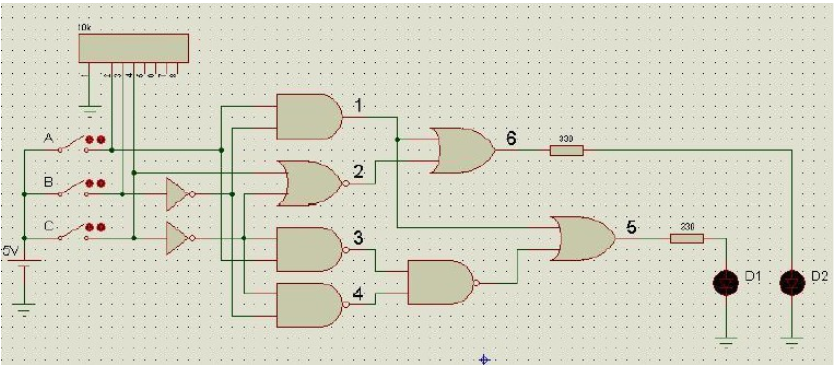
\includegraphics[width=0.8\textwidth]{images/Cap_Circuito.png}
    \caption{Circuito original}
    \label{fig:mi-etiqueta}
\end{figure}

En la imagen podemos apreciar el el circuito cuenta con:
\begin{enumerate}
\item Tres interruptores
\item Un set de resistencias pull-down
\item Dos inversores (NOT)
\item Siete puertas logicas distintas
\item Dos resistencias comunes
\item Dos luces led
\end{enumerate}
Notar que las siete puertas logicas, solo hay seis enumeradas, por lo tanto, desde ahora en mas, por motivos practicos decidimos llamar a dicha puerta logica como `Pureta x`.

La puertas logicas del circuito corresponden a:

\begin{table}[htbp]
    \centering
    \caption{Relación de puertas lógicas.}
    \label{tab:puertas_logicas}
    \begin{tabular}{c|l}
        \hline
        \textbf{Puerta} & \textbf{Lógica} \\ \hline
        1 & AND \\
        2 & NOR \\
        3 & NAND \\
        4 & NAND \\
        5 & OR \\
        6 & OR \\
        x & NAND \\
        \hline
    \end{tabular}
\end{table}


\section{Construcción de la tabla de verdad}

Podemos reconocer que la tabla de verdad posee 3 entradas y 2 salidas, siendo las entradas $\{A, B, C\}$, mientras que las salidas son $\{D1, D2\}$. Con la información anterior podemos deducir que nuestra tabla poseerá ocho hileras, gracias a la relación nombrada en el marco teórico. Asimismo, para detallar el comportamiento completo del circuito y de cada una de sus partes, se han incorporado las funciones intermedias correspondientes a todas las compuertas del diseño original ($F_1$ hasta $F_6$ ademas de $F_X$), quedando estructurada de la siguiente manera:

\begin{table}[H]
    \centering
    \caption{Tabla de verdad extendida con todas las salidas intermedias y principales.}
    \label{tab:tabla-verdad-extendida}
    \begin{tabular}{ccc|ccccccc|cc}
        \toprule
        $A$ & $B$ & $C$ & $F_1$ & $F_2$ & $F_3$ & $F_4$ & $F_5$ & $F_6$ & $F_X$ & $D1$ & $D2$ \\
        \midrule
        0 & 0 & 0 & -- & -- & -- & -- & -- & -- & -- & -- & -- \\
        0 & 0 & 1 & -- & -- & -- & -- & -- & -- & -- & -- & -- \\
        0 & 1 & 0 & -- & -- & -- & -- & -- & -- & -- & -- & -- \\
        0 & 1 & 1 & -- & -- & -- & -- & -- & -- & -- & -- & -- \\
        1 & 0 & 0 & -- & -- & -- & -- & -- & -- & -- & -- & -- \\
        1 & 0 & 1 & -- & -- & -- & -- & -- & -- & -- & -- & -- \\
        1 & 1 & 0 & -- & -- & -- & -- & -- & -- & -- & -- & -- \\
        1 & 1 & 1 & -- & -- & -- & -- & -- & -- & -- & -- & -- \\
        \bottomrule
    \end{tabular}
\end{table}

Por temas de simplicidad, se evito mencionar las puertas logicas (NOT) en la tabla, seran tomadas en cuenta mediante algebra booleana.

\section{Obtención de las funciones booleanas y simplificación mediante álgebra booleana}

A partir del análisis del circuito original, se determinan las funciones lógicas intermedias para cada compuerta y nodo del sistema:

\begin{align*}
    F_1 &= A \overline{B} \\
    F_2 &= \overline{C + \overline{C}} \\
    F_3 &= \overline{A \overline{C}} \\
    F_4 &= \overline{\overline{B} \overline{C}} \\
    F_5 &= F_1 + F_x = A \overline{B} + \left[ (\overline{A \overline{C}}) (\overline{\overline{B} \overline{C}}) \right] \\
    F_6 &= A \overline{B} \ \overline{C + \overline{C}}
\end{align*}

Las simplificaciones con sus respectivas reglas son tal que:

\begin{align*}
    F_2 &= \overline{C + \overline{C}}= \overline{1} = 0 && \text{--- Regla del complemento} \\
    F_3 &= \overline{A \overline{C}}= \overline{A} + \overline{\overline{C}} && \text{--- Ley de Morgan y Doble Negación} \\
    F_4 &= \overline{\overline{B} \overline{C}} = \overline{\overline{B}}+ \overline{\overline{C}} = B + C && \text{--- Ley de Morgan y Doble Negación} \\
    F_5 &= A \overline{B} + \left( \overline{A \overline{C}} \right) \left( \overline{\overline{B} \overline{C}} \right) = A \overline{B} + ( A + C )( B + C ) && \text{--- Ley de Morgan y Doble Negación} \\
    F_6 &= A\overline{B} + 0 = A \overline{B} && \text{--- Identidad}
\end{align*}
\section{Simplificación mediante mapas de Karnaugh}


% ---------------------------------------------------------
% 4.6 Simulación
% ---------------------------------------------------------

\section{Verificación mediante simulación}


% ---------------------------------------------------------
% 4.7 Montaje físico
% ---------------------------------------------------------

\section{Montaje físico del circuito}


% =========================================================
% 5.1 ANÁLISIS DEL CIRCUITO ORIGINAL
% =========================================================

\section{Análisis lógico del circuito original}

% Presentar las expresiones correspondientes
% a cada compuerta o nodo numerado del circuito.
%
% Por ejemplo:
%
% F1 = ...
% F2 = ...
% F3 = ...
% F4 = ...
%
% Utilizar únicamente las expresiones previamente
% revisadas.


% Ejemplo de formato:
%
% \begin{equation}
%     F_1 = ...
% \end{equation}


% =========================================================
% 5.2 TABLA DE VERDAD
% =========================================================

\section{Tabla de verdad}

\begin{table}[H]

    \centering

    \caption{Tabla de verdad del circuito combinacional.}

    \label{tab:tabla-verdad}

    \begin{tabular}{ccc|cc}

        \toprule

        $A$ & $B$ & $C$ & $D1$ & $D2$ \\

        \midrule

        0 & 0 & 0 & -- & -- \\

        0 & 0 & 1 & -- & -- \\

        0 & 1 & 0 & -- & -- \\

        0 & 1 & 1 & -- & -- \\

        1 & 0 & 0 & -- & -- \\

        1 & 0 & 1 & -- & -- \\

        1 & 1 & 0 & -- & -- \\

        1 & 1 & 1 & -- & -- \\

        \bottomrule

    \end{tabular}

\end{table}


\chapter{Conclusiones}\label{conclusion}


%%%%%
%agregar referencias
\bibliographystyle{ieeetr}
%\nocite{*} % mostrar todas las referencias aunque no esten citadas
\bibliography{bibliografia.bib}

\end{document}
